\section{Neural networks}

While the basis for the modern neural network was laid more than a hundred years ago in the late 1800's what we think of in modern terms was proposed by \citet{McCulloch1943}. They propose a computational structure that acts in a fashion like a human neuron. That is it takes input from multiple sources,weights that input and produces an activation if the signal is strong enough. These lose definitions will be made more mathematically clear but for the moment we stick with the simple intuition. Ordinarily a neuron is said to be located in a layer where all the neurons connect to the same input. This layer then produces an output for each neuron in that layer, controlling the output-space of the transformation. A simple illustration of two neurons is provided in figure \ref{fig:ann_illustration}


\tikzset{every picture/.style={line width=0.75pt}} %set default line width to 0.75pt        


\begin{figure}[h]
\centering
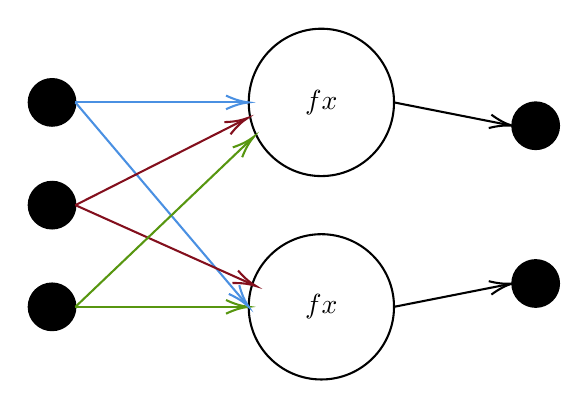
\begin{tikzpicture}[x=0.75pt,y=0.75pt,yscale=-1,xscale=1]
%uncomment if require: \path (0,300); %set diagram left start at 0, and has height of 300

%Flowchart: Connector [id:dp526297050187353] 
\draw   (285,88.5) .. controls (285,68.89) and (300.67,53) .. (320,53) .. controls (339.33,53) and (355,68.89) .. (355,88.5) .. controls (355,108.11) and (339.33,124) .. (320,124) .. controls (300.67,124) and (285,108.11) .. (285,88.5) -- cycle ;
%Flowchart: Connector [id:dp5646385359122916] 
\draw   (285,187) .. controls (285,167.67) and (300.67,152) .. (320,152) .. controls (339.33,152) and (355,167.67) .. (355,187) .. controls (355,206.33) and (339.33,222) .. (320,222) .. controls (300.67,222) and (285,206.33) .. (285,187) -- cycle ;
%Flowchart: Connector [id:dp3104075761318521] 
\draw  [fill={rgb, 255:red, 0; green, 0; blue, 0 }  ,fill opacity=1 ] (179,88.5) .. controls (179,82.29) and (184.04,77.25) .. (190.25,77.25) .. controls (196.46,77.25) and (201.5,82.29) .. (201.5,88.5) .. controls (201.5,94.71) and (196.46,99.75) .. (190.25,99.75) .. controls (184.04,99.75) and (179,94.71) .. (179,88.5) -- cycle ;
%Flowchart: Connector [id:dp15106578289314898] 
\draw  [fill={rgb, 255:red, 0; green, 0; blue, 0 }  ,fill opacity=1 ] (179,187) .. controls (179,180.79) and (184.04,175.75) .. (190.25,175.75) .. controls (196.46,175.75) and (201.5,180.79) .. (201.5,187) .. controls (201.5,193.21) and (196.46,198.25) .. (190.25,198.25) .. controls (184.04,198.25) and (179,193.21) .. (179,187) -- cycle ;
%Flowchart: Connector [id:dp06829960407828417] 
\draw  [fill={rgb, 255:red, 0; green, 0; blue, 0 }  ,fill opacity=1 ] (179,138) .. controls (179,131.79) and (184.04,126.75) .. (190.25,126.75) .. controls (196.46,126.75) and (201.5,131.79) .. (201.5,138) .. controls (201.5,144.21) and (196.46,149.25) .. (190.25,149.25) .. controls (184.04,149.25) and (179,144.21) .. (179,138) -- cycle ;
%Straight Lines [id:da16938395812882923] 
\draw [color={rgb, 255:red, 74; green, 144; blue, 226 }  ,draw opacity=1 ]   (201.5,88.5) -- (283,88.5) ;
\draw [shift={(285,88.5)}, rotate = 180] [color={rgb, 255:red, 74; green, 144; blue, 226 }  ,draw opacity=1 ][line width=0.75]    (10.93,-3.29) .. controls (6.95,-1.4) and (3.31,-0.3) .. (0,0) .. controls (3.31,0.3) and (6.95,1.4) .. (10.93,3.29)   ;

%Straight Lines [id:da6971592528694486] 
\draw [color={rgb, 255:red, 87; green, 150; blue, 16 }  ,draw opacity=1 ][fill={rgb, 255:red, 0; green, 0; blue, 0 }  ,fill opacity=1 ]   (201.5,187) -- (283,187) ;
\draw [shift={(285,187)}, rotate = 180] [color={rgb, 255:red, 87; green, 150; blue, 16 }  ,draw opacity=1 ][line width=0.75]    (10.93,-3.29) .. controls (6.95,-1.4) and (3.31,-0.3) .. (0,0) .. controls (3.31,0.3) and (6.95,1.4) .. (10.93,3.29)   ;

%Straight Lines [id:da7906184612815319] 
\draw [color={rgb, 255:red, 74; green, 144; blue, 226 }  ,draw opacity=1 ]   (201.5,88.5) -- (283.71,185.47) ;
\draw [shift={(285,187)}, rotate = 229.71] [color={rgb, 255:red, 74; green, 144; blue, 226 }  ,draw opacity=1 ][line width=0.75]    (10.93,-3.29) .. controls (6.95,-1.4) and (3.31,-0.3) .. (0,0) .. controls (3.31,0.3) and (6.95,1.4) .. (10.93,3.29)   ;

%Straight Lines [id:da1362874028964085] 
\draw [color={rgb, 255:red, 131; green, 15; blue, 29 }  ,draw opacity=1 ][fill={rgb, 255:red, 0; green, 0; blue, 0 }  ,fill opacity=1 ]   (201.5,138) -- (282.72,96.9) ;
\draw [shift={(284.5,96)}, rotate = 513.1600000000001] [color={rgb, 255:red, 131; green, 15; blue, 29 }  ,draw opacity=1 ][line width=0.75]    (10.93,-3.29) .. controls (6.95,-1.4) and (3.31,-0.3) .. (0,0) .. controls (3.31,0.3) and (6.95,1.4) .. (10.93,3.29)   ;

%Straight Lines [id:da569846296368284] 
\draw [color={rgb, 255:red, 131; green, 15; blue, 29 }  ,draw opacity=1 ][fill={rgb, 255:red, 0; green, 0; blue, 0 }  ,fill opacity=1 ]   (201.5,138) -- (286.67,176.18) ;
\draw [shift={(288.5,177)}, rotate = 204.15] [color={rgb, 255:red, 131; green, 15; blue, 29 }  ,draw opacity=1 ][line width=0.75]    (10.93,-3.29) .. controls (6.95,-1.4) and (3.31,-0.3) .. (0,0) .. controls (3.31,0.3) and (6.95,1.4) .. (10.93,3.29)   ;

%Straight Lines [id:da6518887295694358] 
\draw [color={rgb, 255:red, 87; green, 150; blue, 16 }  ,draw opacity=1 ][fill={rgb, 255:red, 0; green, 0; blue, 0 }  ,fill opacity=1 ]   (201.5,187) -- (286.05,106.38) ;
\draw [shift={(287.5,105)}, rotate = 496.36] [color={rgb, 255:red, 87; green, 150; blue, 16 }  ,draw opacity=1 ][line width=0.75]    (10.93,-3.29) .. controls (6.95,-1.4) and (3.31,-0.3) .. (0,0) .. controls (3.31,0.3) and (6.95,1.4) .. (10.93,3.29)   ;

%Flowchart: Connector [id:dp5234386771770392] 
\draw  [fill={rgb, 255:red, 0; green, 0; blue, 0 }  ,fill opacity=1 ] (412,99.75) .. controls (412,93.54) and (417.04,88.5) .. (423.25,88.5) .. controls (429.46,88.5) and (434.5,93.54) .. (434.5,99.75) .. controls (434.5,105.96) and (429.46,111) .. (423.25,111) .. controls (417.04,111) and (412,105.96) .. (412,99.75) -- cycle ;
%Flowchart: Connector [id:dp4431827599012259] 
\draw  [fill={rgb, 255:red, 0; green, 0; blue, 0 }  ,fill opacity=1 ] (412,175.75) .. controls (412,169.54) and (417.04,164.5) .. (423.25,164.5) .. controls (429.46,164.5) and (434.5,169.54) .. (434.5,175.75) .. controls (434.5,181.96) and (429.46,187) .. (423.25,187) .. controls (417.04,187) and (412,181.96) .. (412,175.75) -- cycle ;
%Straight Lines [id:da8359806786193378] 
\draw    (355,88.5) -- (410.04,99.36) ;
\draw [shift={(412,99.75)}, rotate = 191.16] [color={rgb, 255:red, 0; green, 0; blue, 0 }  ][line width=0.75]    (10.93,-3.29) .. controls (6.95,-1.4) and (3.31,-0.3) .. (0,0) .. controls (3.31,0.3) and (6.95,1.4) .. (10.93,3.29)   ;

%Straight Lines [id:da2250239797689928] 
\draw    (355,187) -- (410.04,176.14) ;
\draw [shift={(412,175.75)}, rotate = 528.8399999999999] [color={rgb, 255:red, 0; green, 0; blue, 0 }  ][line width=0.75]    (10.93,-3.29) .. controls (6.95,-1.4) and (3.31,-0.3) .. (0,0) .. controls (3.31,0.3) and (6.95,1.4) .. (10.93,3.29)   ;


% Text Node
\draw (320,88.5) node   {$fx$};
% Text Node
\draw (320,187) node   {$fx$};
\end{tikzpicture}
\caption{An illustration of the graph constructed by two artificial neurons with three input nodes. Colored lines illustrate that  each of the input nodes are connected to each of the neurons in a manner we denote as fully-connected.}\label{fig:ann_illustration}
\end{figure}


\noindent To formalize this idea let the input be $x \in \R^N$, let then the matrix $W \in \R^{N \times D}$ be the representation of the weight matrix forming the connenctions between the input and the artificial neurons. Lastly we define the activation function $f(x)$ as a univariate, monotonic function on $\R^1$. We will explore this function in some detail later. A layer in a network implements what we will call a forward pass as defined in function \ref{eq:fwd}.

\begin{equation}\label{eq:fwd}
\hat{y} = f(\inner{x}{W}_D)
\end{equation}

In equation \ref{eq:fwd} the subscript denotes that the function is applied element-wise and we denote the inner product in bra-ket notation with $\inner{\cdot}{\cdot}$. Each node is aditionally associated with a bias node ensuring that even zeroed-cells can encode information. Let the bias for the layer be given as $b \in \R^D$ in keeping with the notation above. Equation \ref{eq:fwd} then becomes as presented in equation \ref{eq:fwd_b}

\begin{equation}\label{eq:fwd_b}
\hat{y} = f(\inner{x}{W}_D) + b
\end{equation}

As a tie to more traditional methods we note that in the face of the identity transform $f(x) = x$ the equation \ref{eq:fwd_b} becomes the formulation for a linear regression model. In our model the variables that need to be fit are the elements of $W$ that we denote $\wij$. What remains then is  to formulate a loss function w.r.t the intended output $y$ that we will denote as $\mathcal{L}(y, \hat{y}, W)$. Based on whether the output is described by real values, or a set of probabilities this function, $\loss$, takes on the familiar form of the Mean Squared Error or in the event that we want to estimate the likelihood of the output under the data; the binary crossentropy. We will also explore these functions in some detail later. To find the optimal values for $\wij$ we then formulate a gradient optimization like in equation \ref{eq:gd}

\begin{equation}\label{eq:gd}
\wij \leftarrow -\eta \frac{\partial \loss}{\partial \wij} + \wij 
\end{equation}